\documentclass[a4paper,twocolumn,twoside,10pt]{book}
\usepackage[utf8x]{inputenc}
\usepackage[a4paper,margin=1in]{geometry}
%\usepackage{fancyhdr}
\usepackage{pdfpages}
\usepackage{url}
\pagestyle{plain}

\begin{document}

\title{Proceedings of the \\ Second International Go Game Science Conference}
\author{IGGSC2015 \\ Petr Baudiš, Josef Moudřík (eds.)}
\date{July 29--30, 2015 \\ EGC2015 in Liberec, Czech Republic}

\frontmatter
\maketitle

%% copyrightpage
\begingroup
\pagestyle{empty}
\footnotesize
\parindent 0pt
\parskip \baselineskip

~

\subsubsection{Organizing Committee}
\noindent
Josef Moudřík

\noindent
Petr Baudiš

\noindent
Pawel Noga

\vskip 5ex

\subsubsection{Program Committee}
\noindent
\textit{members of the organizing committee, and:}

\noindent
Martin Müller

\noindent
Peter Shotwell

\noindent
Thomas Wolf


\vskip 30ex

The papers printed in these proceedings are also available online
at \url{http://pasky.or.cz/iggsc2015/} in color or with additional
appendices.

The papers are \textcopyright{} of their respective authors,
and are made available under the terms of the Creative Commons
licence Attribution-NoDerivatives 4.0 International (CC-BY-ND).

\vfill


\noindent
Published by MATFYZPRESS\\
Publishing House of the Faculty of Mathematics and Physics,
Charles University in Prague\\
Sokolovská 83, 186 75 Praha 8, Czech Republic\\
as 493rd publication.\\
The publication did not undergo MFF review process.\\
Printed by Reprostředisko UK MFF,\\
Sokolovská 83, 186 75 Praha 8, Czech Republic.\\
First edition\\
Prague 2015\\

\noindent
ISBN 978-80-7378-299-3

%%%%{\LARGE\plogo}
\vspace*{2\baselineskip}


\endgroup
\clearpage


\chapter*{Introduction}

Dear Reader,

You are holding a~printed proceedings of the Second International Go
Game Conference, taking place in Liberec, Czech Republic, as a~part of
European Go Congress 2015.

The aim of the conference is to share knowledge between researchers
and to show the game of Go from (hopefully) interesting and new point
of view to the general Go public visiting the congress.  The numeral in
the conference name has been chosen to be ''Second'' to promote the idea
of Science Conferences on Go Congresses, which -- to our knowledge --
started on 2013's congress in Olsztyn, Poland. We sincerely hope that this
newly-founded tradition will continue in the forthcoming years as well.

In this proceedings, you will find the four conference
submissions. Despite all our effort, we were obviously unable to attract
many authors; our conclusion is that it was probably a mistake being so
formal with publication process and visual style. Nevertheless, we still
hope you will enjoy both reading the papers and the conference itself.

The conference would not be possible without our program committee members
Martin Müller, Peter Shotwell and Thomas Wolf, thank You. Finally,
we would like to thank our sponsor, mathematician and philanthropist
Karel Janeček.

\vspace*{2ex}
\noindent On behalf of the Organizing Committee,\newline Josef Moudřík,
Summer 2015.

\tableofcontents

\mainmatter

\cleardoublepage
\addcontentsline{toc}{chapter}{Computer-Aided Go on High-dan Level \protect\newline (Ingo Althöfer, Manja Marz, Stefan Kaitschik)}
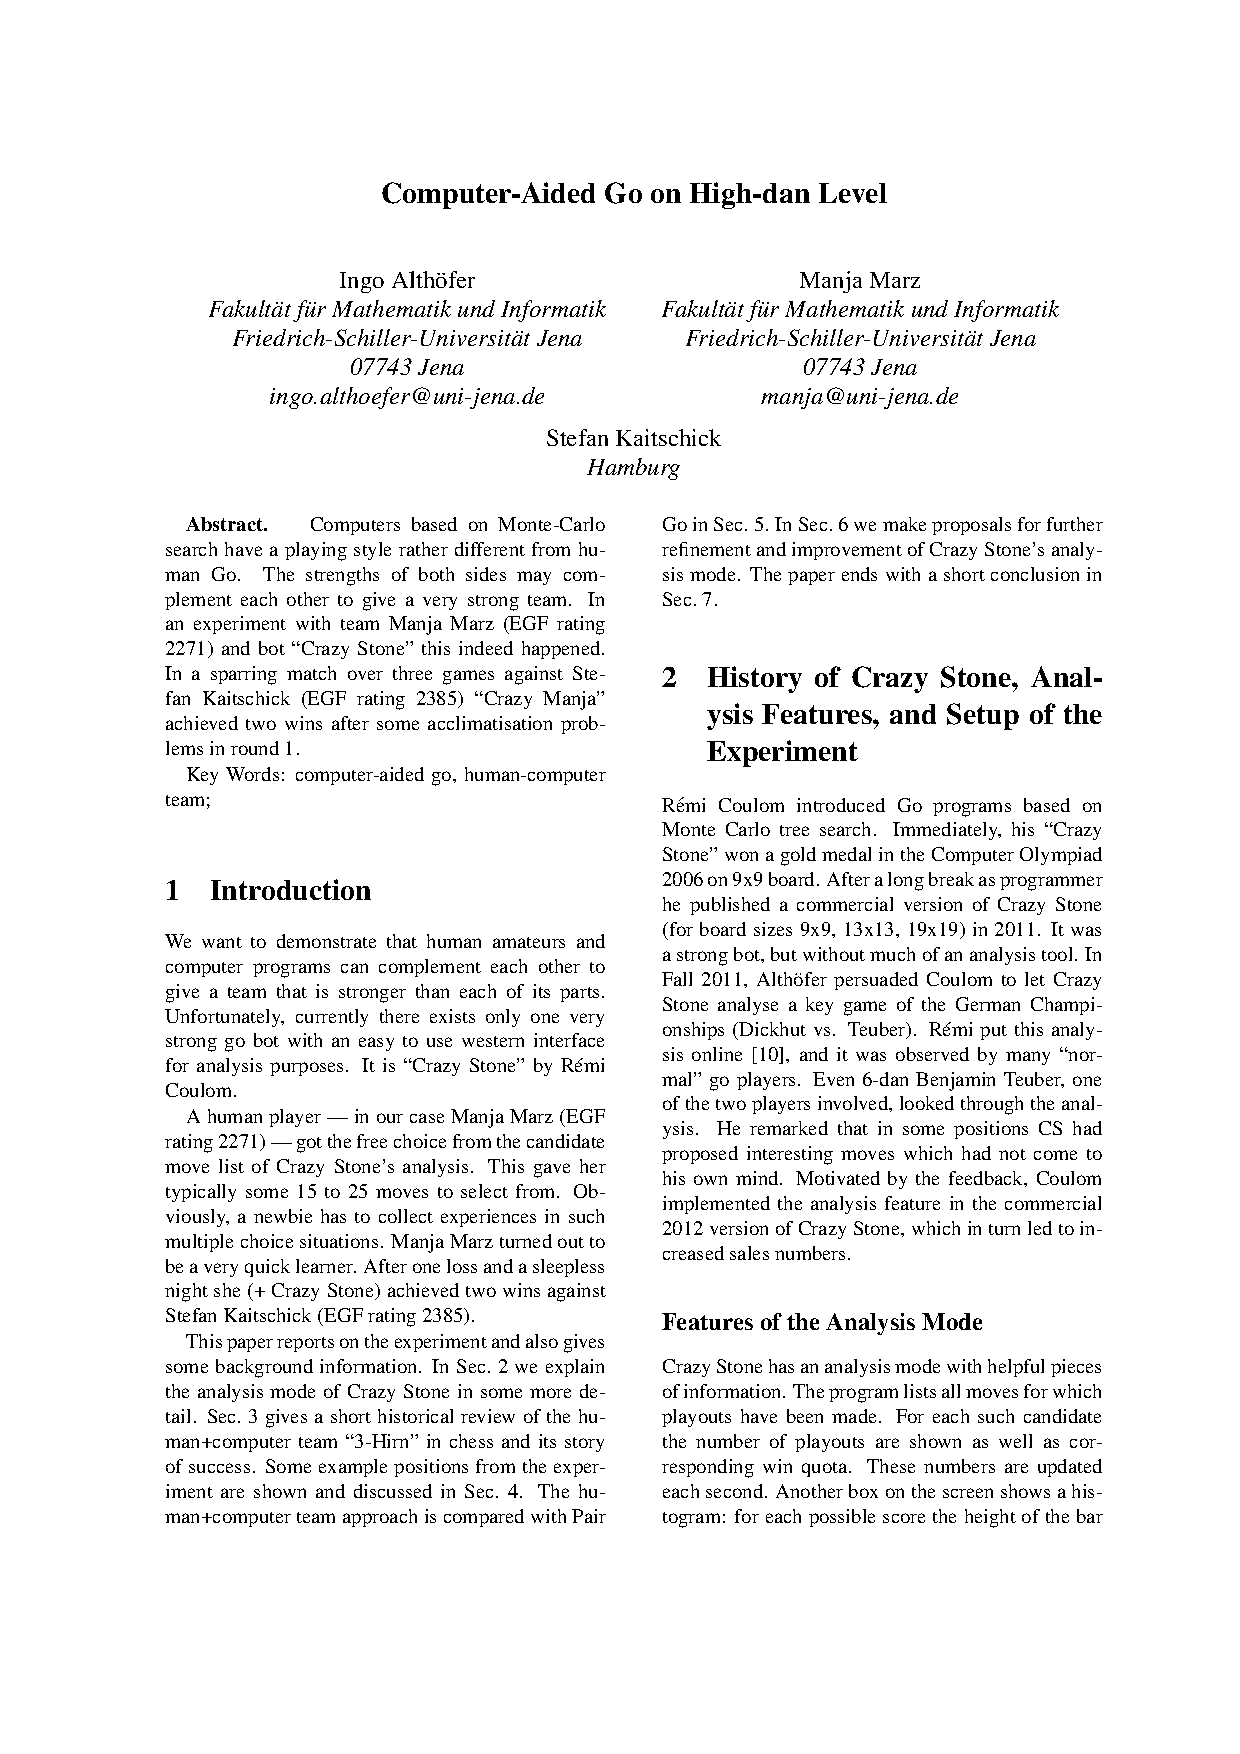
\includepdf[pages=-,pagecommand={\pagestyle{plain}}]{Althoefer.pdf}

\cleardoublepage
\addcontentsline{toc}{chapter}{A New Approach to an Old Problem: The Reconstruction \protect\newline of a Go Game through a Series of Photographs \protect\newline (Andrea Carta, Mario Corsolini)}
\includepdf[pages=1-12,pagecommand={\pagestyle{plain}}]{Carta-Corsolini.pdf}

\cleardoublepage
\addcontentsline{toc}{chapter}{A Proposal of Global Open Data Index for the Game of Go \protect\newline (Leonardo Alberto Dal Zovo, Angela Corbari)}
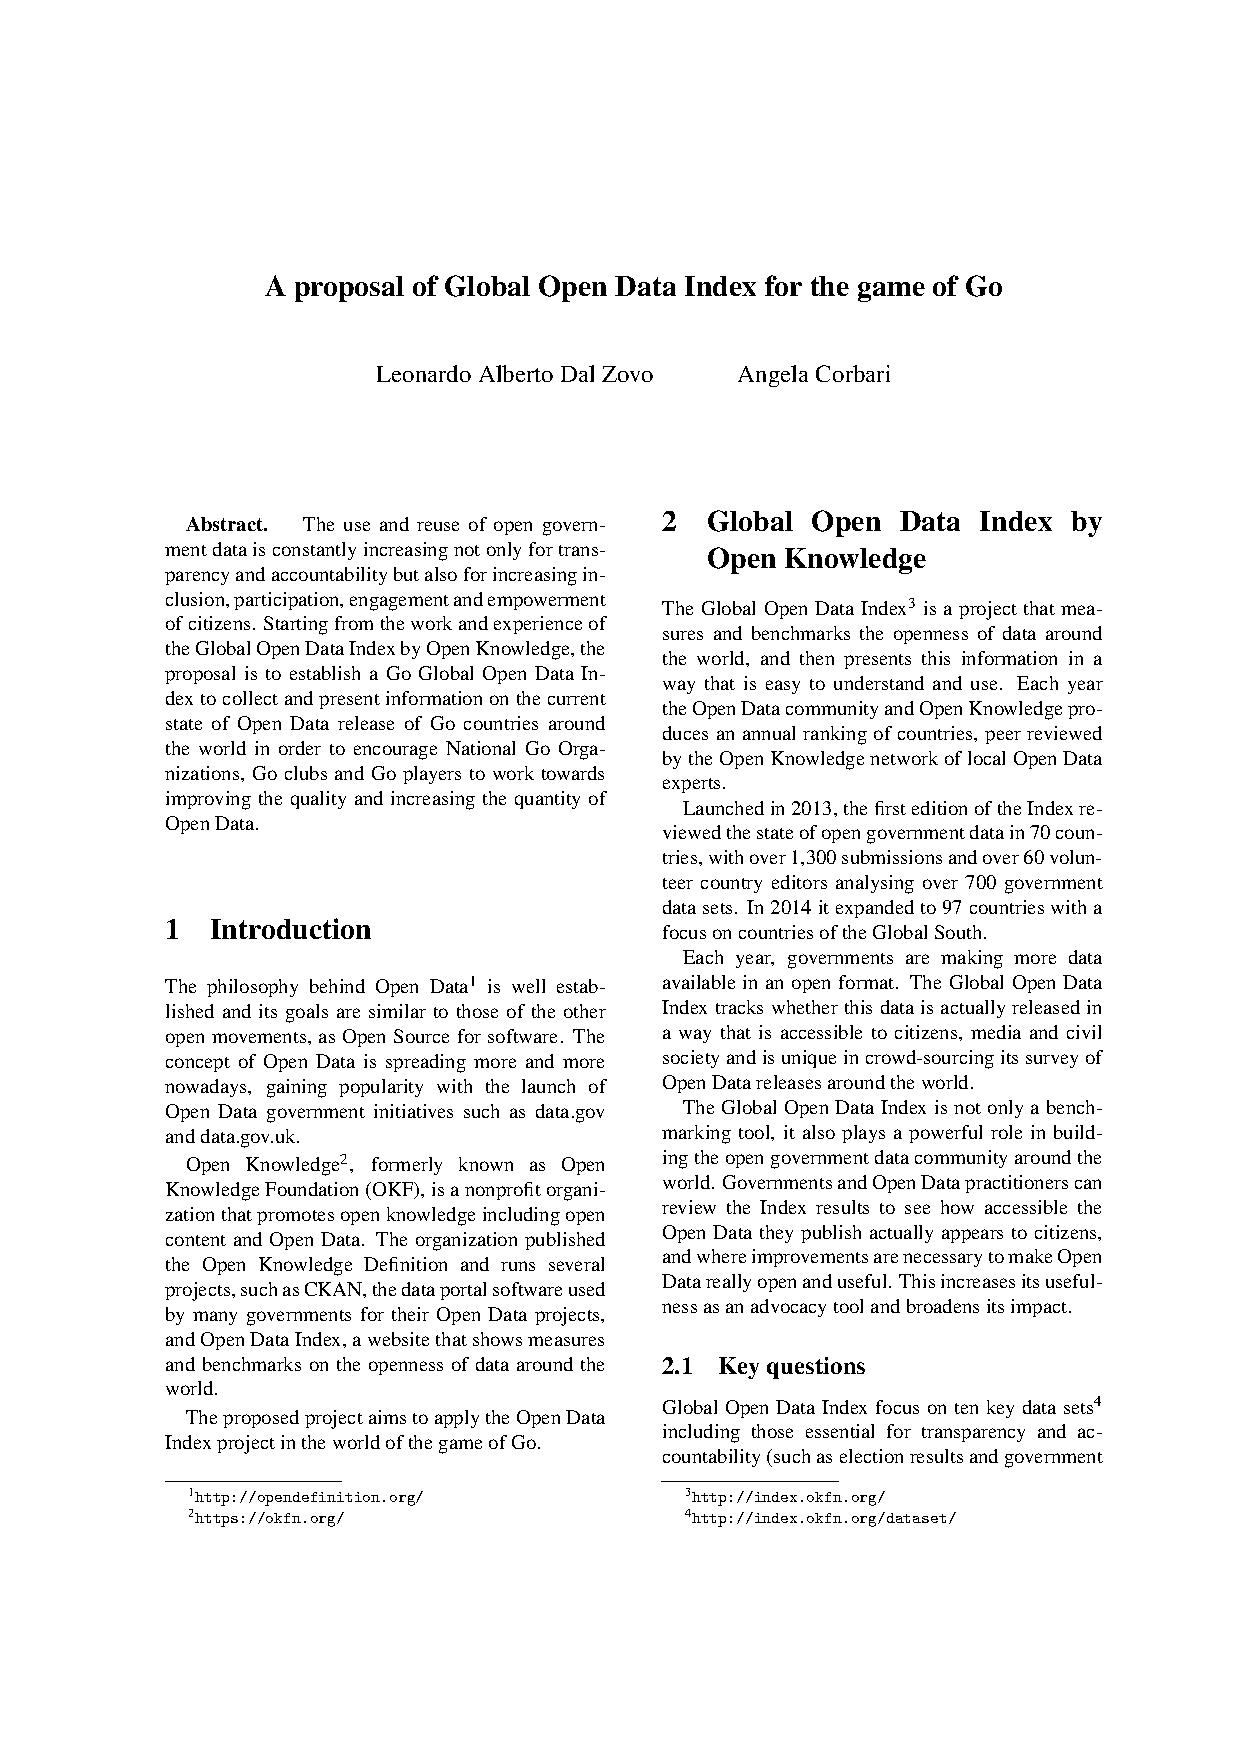
\includepdf[pages=-,pagecommand={\pagestyle{plain}}]{DelZovo.pdf}

\cleardoublepage
\addcontentsline{toc}{chapter}{Improving Learning Progress in a Mind Sport Game \protect\newline (Marc Oliver Rieger, Stefan Rössel)}
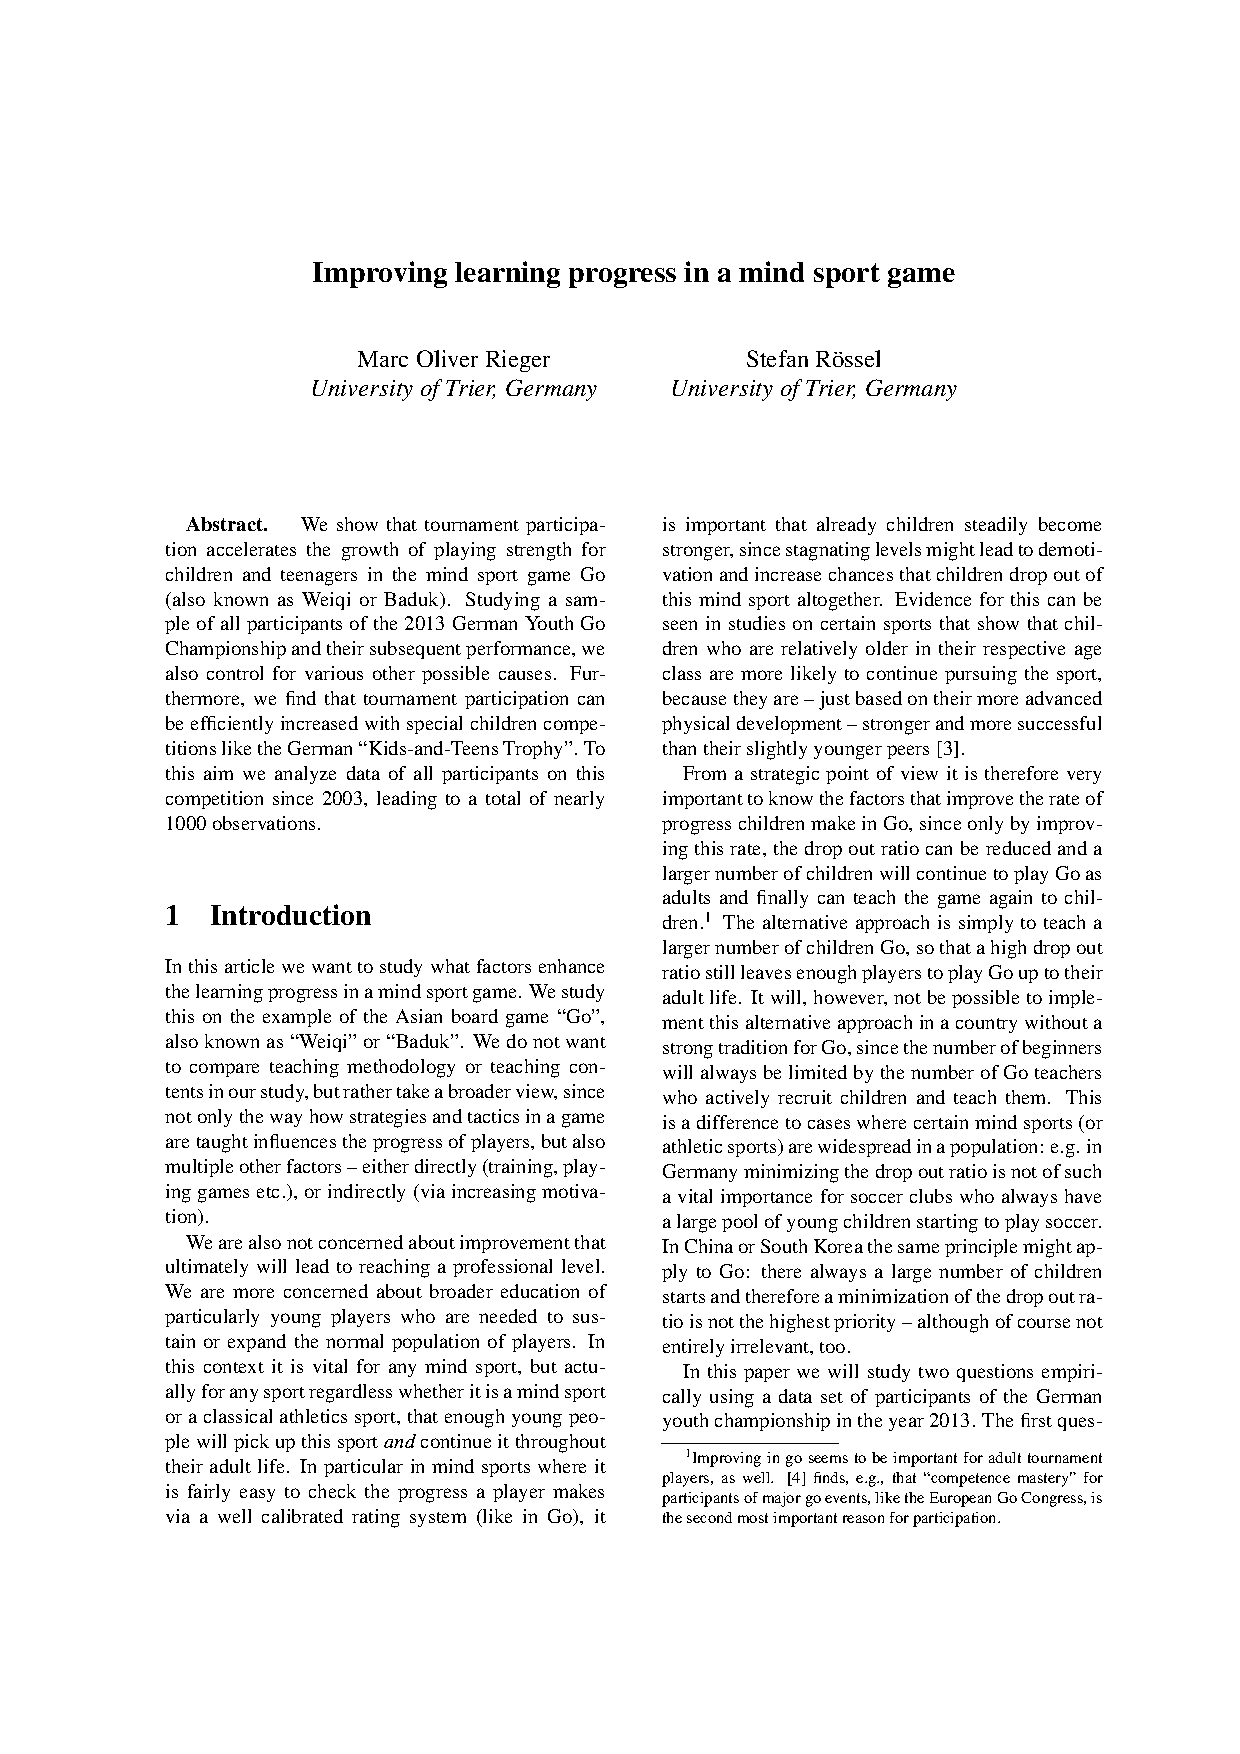
\includepdf[pages=-,pagecommand={\pagestyle{plain}}]{Rieger.pdf}

\end{document}
